\renewcommand{\NomeBloco}{\emph{APS\_pixel\_clk}}
\renewcommand{\NomeBlocoNoUnderline}{apspixelclk}
\renewcommand{\NomePTab}{tab_\NomeBlocoNoUnderline}
\renewcommand{\NomeSTab}{tab_\NomeBlocoNoUnderline2}
\renewcommand{\NomePFig}{fig_\NomeBlocoNoUnderline}
\renewcommand{\NomeSFig}{fig_\NomeBlocoNoUnderline2}
\renewcommand{\NomeTTab}{tab_\NomeBlocoNoUnderline3}
\renewcommand{\NomeQTab}{tab_\NomeBlocoNoUnderline4}

\section{\NomeBloco}

O \NomeBloco{} \'e o bloco respons\'avel por processar e digitalizar o sinal gerado pelo \emph{TIA}. A inten{\c c}\~ao de uso do \emph{TIA} \'e que ele seja o respons\'avel por captar um sinal luminoso com frequ\^encia bem definida, e o sinal el\'etrico gerado, em forma de pulsos quadrados, sirva de refer\^encia de rel\'ogio para todos os circuitos APS utilizados para detec{\c c}\~ao de cor. O bloco portanto tem como responsabilidade gerar um sinal digital de frequ\^encia igual \'a do sinal luminoso captado. O bloco apresenta as defini{\c c}\~oes de sinais de entrada e sa\'ida referidos na \autoref{\NomeSTab}.

\begin{table}[htbp]
\caption{Sinais do bloco \NomeBloco}
\label{\NomeSTab}
\centering
\begin{tabular}{ccl}

    \toprule
    Sinal & Tipo    & Descri{\c c}\~ao\\
    \midrule \midrule
    Vref\_comp   & Entrada   & Tens\~ao de refer\^encia utilizada pelo comparador\\
    \midrule
    Vref\_amp   & Entrada   & Tens\~ao de refer\^encia utilizada para o TIA\\
    \midrule
    Ibias   & Entrada   & Corrente de polariza{\c c}\~ao do comparador \\
    \midrule
    Vout   & Saída   & Sinal digital produzido pelo Comparador\\
    \bottomrule
\end{tabular}
\legend{Fonte: Produzido pelo autor}
\end{table}

O circuito projetado para o bloco \'e demonstrado na \autoref{\NomePFig}.

\begin{figure}[htb]
 \centering
    \centering
    \caption{Circuito CMOS projetado para o bloco \NomeBloco} 
    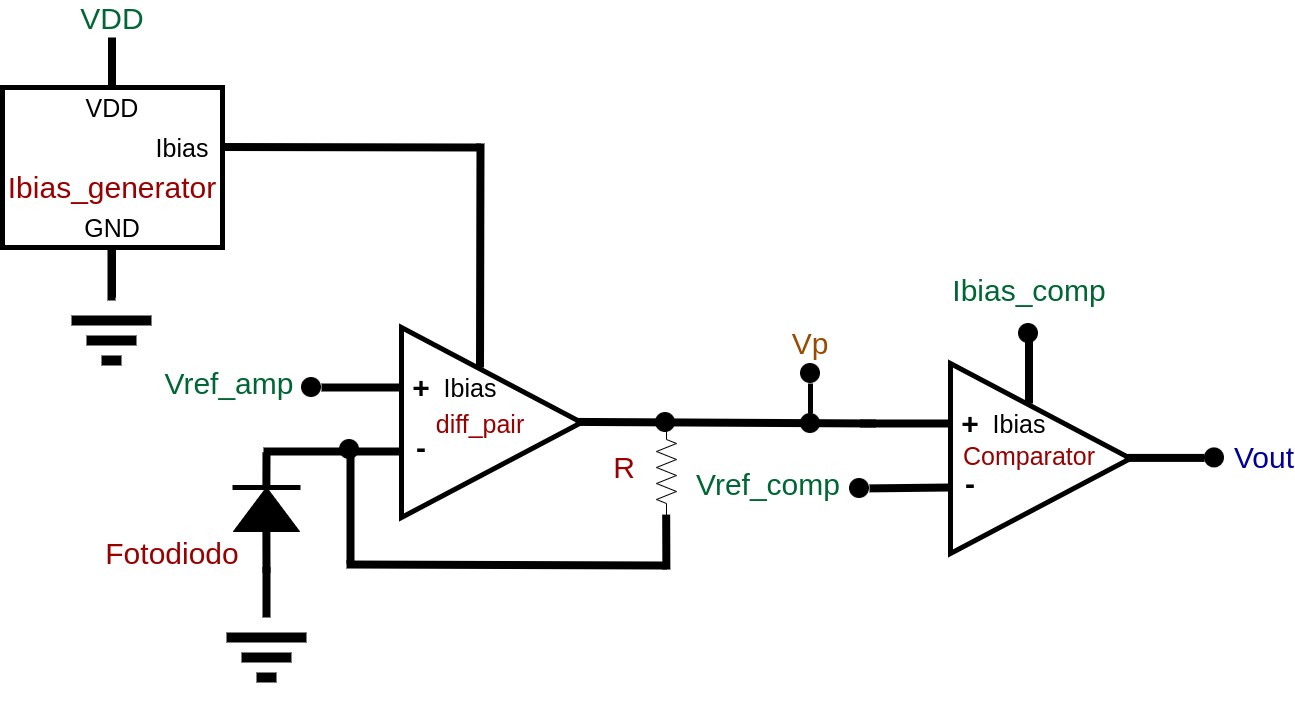
\includegraphics[scale=0.3]{Circuitos/APS_clk.png}
    \label{\NomePFig}
    \legend{Fonte: Produzido pelo autor}
\end{figure}

\begin{figure}[htb]
 \centering
    \centering
    \caption{Representa{\c c}\~ao em bloco do \NomeBloco} \label{\NomeSFig}
    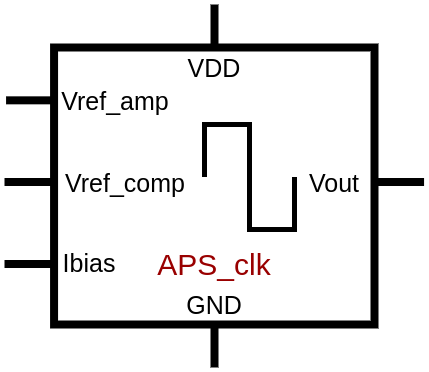
\includegraphics[scale=0.3]{Circuitos/APS_clk_block.png}
    \legend{Fonte: Produzido pelo autor}
\end{figure}

O circuito tem funcionamento similar ao do apresentado no bloco \emph{APS\_digitalized}, por\'em com apenas a sa\'ida digital sendo considerada e sendo utilizado um $TIA$ ao inv\'es de um \emph{APS}. A corrente de polariza{\c c}\~ao do par diferencial \'e gerada pelo bloco \emph{Ibias\_generator}, contido no bloco.

Uma resist\^encia $R$ de ganho \'e utilizada, com valor apresentado na \autoref{\NomeQTab}.

\begin{table}[htb]
\caption{Resistor do bloco \NomeBloco}
\label{\NomeQTab}
\centering
\begin{tabular}{cccc}
\toprule
Resistor & W ($\mu$m)  & L ($\mu$m) & Resist\^encia (M$\Omega$)\\
\midrule \midrule
R & 1,68 & 39486,3 & 25\\
\bottomrule
\end{tabular}
\legend{Fonte: Produzido pelo autor}
\end{table}

Considerando $R_{sh}$ do fotodiodo tendendo ao infinito e com base na \autoref{eqCTIA}, a \autoref{eq_TIAblock} descreve $V_{p}$, que \'e comparada com \emph{Vref\_comp} e ent\~ao utilizada para gerar o sinal de sa\'ida.

\begin{equation}
    \label{eq_TIAblock}
    V_{p} = RI_{PH} + V_{ref\_amp}
\end{equation}

Onde:

\begin{itemize}

    \item \emph{$V_{PH}$} \'e a tens\~ao no ramo positivo do comparador [$V$]
    \item \emph{$I_{PH}$} \'e a corrente fotogerada [$A$]
    
\end{itemize}